\chapter{Prevádzka a bezpečnosť sietí}
\phantomsection
Prevádzka sieťových zariadení je proces nielen o monitorovaní incidentov, zabezpečovaní konzistencie a konvergencie siete, ale aj o aktualizáciách softvéru a hardvéru, aplikovaní bezpečnostných zásad a politík. Táto kapitola preto opisuje jednotlivé aspekty s ktorými sa pri prevádzke siete môžeme stretnúť.

\section{Sieťové prvky}
\label{hierarchicky-model}
Medzi základné stavebné piliere sietí, bez ktorých nie je možná komunikácia koncových staníc patria smerovače (router) a prepínače (switch). Mimo týchto dvoch základných zariadení sa v \zkratka{zkLAN} sieťach často vyskytujú prístupové body (access point), firewally, sieťové mosty (bridge) a v dnes už ojedinelých prípadoch ešte aj rozbočovače (hub). V súčasnosti však jedno zariadenie môže kombinovať funkcie zariadení, ktoré majú podľa modelov TCP/IP alebo ISO/OSI na starosti inú vrstvu modelu. Preto sa dnes hlavne z finančných dôvodov používajú takzvané L3 prepínače, ktoré s určitými obmedzeniami vedia nahradiť nákladné smerovače. Taktiež smerovače ako aj L3 prepínače umožňujú filtrovanie paketov, takže vedia čiastočne zastať aj základné funkcie firewallu. Značky najpoužívanejších sieťových zariadení su vyobrazené na obrázku \ref{fig:net-devices} a budú používané v nasledujúcich kapitolách.

\begin{figure}[H]
	\begin{center}
		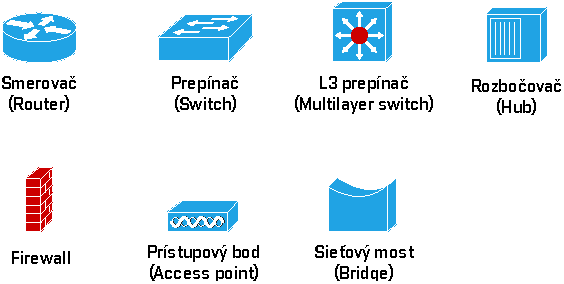
\includegraphics[scale=0.4]{obrazky/net_devices.pdf}
	\end{center}
	\vspace{-5em}
	\caption[Typy sieťových zariadení v lokálnych sieťach]{Typy sieťových zariadení v lokálnych sieťach}
	\label{fig:net-devices}
\end{figure} 

\section{Hierarchický model sietí}
%TODO EDGE
S postupným nárastom sieťových zariadení a komplexnosti siete dochádza v sieťach bez hierarchie k mnohým problémom ako veľké broadcast domény, vysoká cena za port, vysoké zaťaženia zariadení, neprítomnosť redundancie. Preto sa zaviedol hierarchický model siete, ktorý rieši problémy veľkosti a rozsahu broadcast a kolíznych domén, umožňuje efektívne prideľovanie \zkratka{zkIP} adries a oddeľuje zariadenia pracujúce na jednotlivých vrstvách ISO/OSI.  
\\\\
\noindent
Siete sú spravidla delené do 3 vrstiev s definovanými funkciami \cite{Lammle2013}:
\begin{itemize}
	\item Core\,--\,tvorí vysokorýchlostnú chrbticu siete, agreguje dáta z distribučnej vrstvy a mala by byť redundantná. Nároky na rýchlosť portov a výkon zariadenia sú obzvlášť vysoké, a preto sa využívajú prevažne smerovače, ale taktiež ako v distribučnej vrstve dnes už aj L3 prepínače.
	\item Distribučná (Distribution)\,--\,agreguje dáta z prístupovej vrstvy, vytvára a oddeľuje broadcast domény, riadi smerovanie medzi \zkratka{zkVLAN} a  filtrovanie paketov. Táto vrstva kvôli zabezpečeniu dostupnosti využíva agregovanie  a redundanciu liniek. Typicky sa skladá zo smerovačov, no v dnešnej dobe hlavne z L3 prepínačov, keďže tie nie sú finančne také náročné. 
	\item Prístupová (Access)\,--\,vstupný bod do siete, ktorý riadi prístup a politiku pre koncové zariadenia, segmentuje sieť, vytvára a separuje kolízne domény. V neposlednej rade zariaďujú prístup k distribučnej vrstve. Je tvorená zariadeniami ako prepínač, rozbočovač alebo prístupový bod.
\end{itemize} 

\begin{figure}[H]
	\begin{center}
		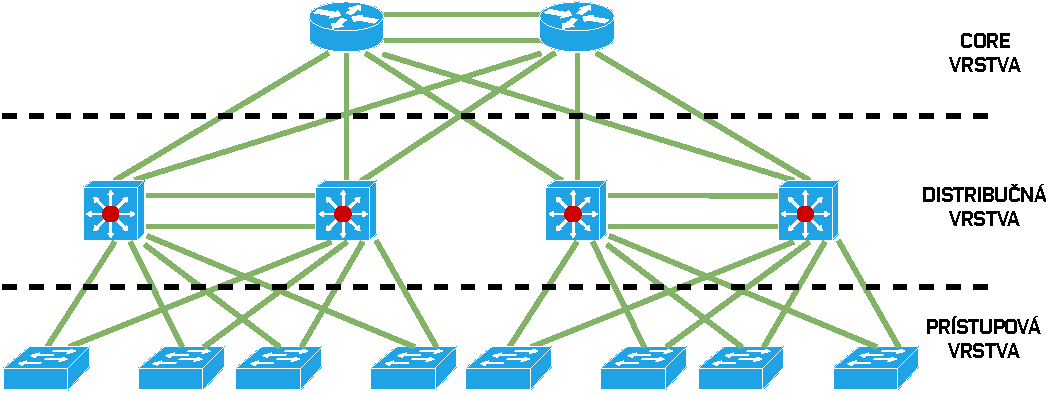
\includegraphics[scale=0.58]{obrazky/hierarchy_network.pdf}
	\end{center}
	\vspace{-11em}
	\caption[Hierarchické rozdelenie siete na vrstvy]{Hierarchické rozdelenie siete na vrstvy}
	\label{fig:net-devices}
\end{figure} 

\noindent
\vspace{2em}
V menších sieťach prevažne malých firiem sa využíva zlučovanie vrstiev nazývaných ako collapsed core, ktoré zlučujú distribučnú a core vrstvu, prípadne zlučujú všetky tri vrstvy dokopy. 

Cieľom hierarchického modelu a dobre navrhnutej siete je dosiahnutie nasledujúcich vlastností:

\begin{itemize}
	\item Škálovateľnosť\,--\,jednoduché a bezproblémové pridanie zariadenia pri raste a rozširovaní siete.
	\item Redundancia\,--\,zabezpečenie vysokej dostupnosti viacnásobnými linkami medzi zariadeniami a zálohovanie samotných zariadení ich redundanciou.
	\item Výkonnosť\,--\,agregovanie liniek a výber dostatočne výkonných zariadení
	\item Bezpečnosť\,--\,zabezpečenie siete na viacerých úrovniach ako napríklad portoch, oddelením segmentov pomocou VLAN, riadením prístupu, šifrovaním a pod.
	\item Manažovateľnosť\,--\,vytvorenie šablón, definovaných štandardov a pravidiel na zaistenie konzistentnosti konfigurácií zariadení na jednoduchšie odhaľovanie chýb. 
	\item Udržovateľnosť\,--\,schopnosť systému prechádzať zmenami komponentov, služieb a vlastností.
\end{itemize}



\section{Funkčné roviny sieťových prvkov}
Sieťové prvky sú zodpovedné nielen za preposielanie dát medzi koncovými stanicami, ale aj za mnohé riadiace dáta medzi sebou, bez ktorých by sieť nebola funkčná. Preto sa jednotlivé protokoly a služby rozdeľujú troch rovín, a to management, control a data plane. Tieto pojmy sa využívajú vo väčšej miere v softvérovo definovaných sieťach, no sú platné aj v klasickej koncepcii.
 
Rovina management je zodpovedná za konfiguráciu a správu zariadení a riadenie prístupu ku konfiguráciám. Typickými príkladmi protokolov pracujúcich na tejto rovine sú \zkratka{zkSNMP}, \zkratka{zkAAA}, Syslog, \zkratka{zkSSH} a mnohé ďalšie \cite{Singh2018}. Druhá rovina, control plane má na starosti prevažne riadenie siete a smerovanie. Zaoberá sa otázkou kadiaľ budú pakety smerované a prenáša riadiace a signalizačné informácie pre protokoly ako napríklad, \zkratka{zkOSPF}, Spanning tree, \zk{zkFHRP} \cite{Singh2018}. Poslednou rovina je data plane nazývaná často aj forwarding plane, ktorá prepína pakety na daný port na základe rozhodnutia z control plane. Táto časť sieťových prvkov musí byť veľmi rýchla, aby zaistila nízku odozvu a dostatočne vysoké prenosové rýchlosti. Nižšie uvedený obrázok \ref{fig:sdn-planes} reflektuje tok dát z jednej roviny do druhej a tiež medzi dvoma susednými zariadeniami. Rovina management plane zodpovedná za konfiguráciu zariadenia a nastavuje rovina control plane, v tomto prípade smerovanie z zariadení. Po výmene informácií so susednými smerovačmi sa vytvoria príslušné tabuľky a nakoniec smerovacia tabuľka, ktorá sa využíva pri rozhodovaní prepínania paketov v revine data plane.

\begin{figure}[H]
	\begin{center}
		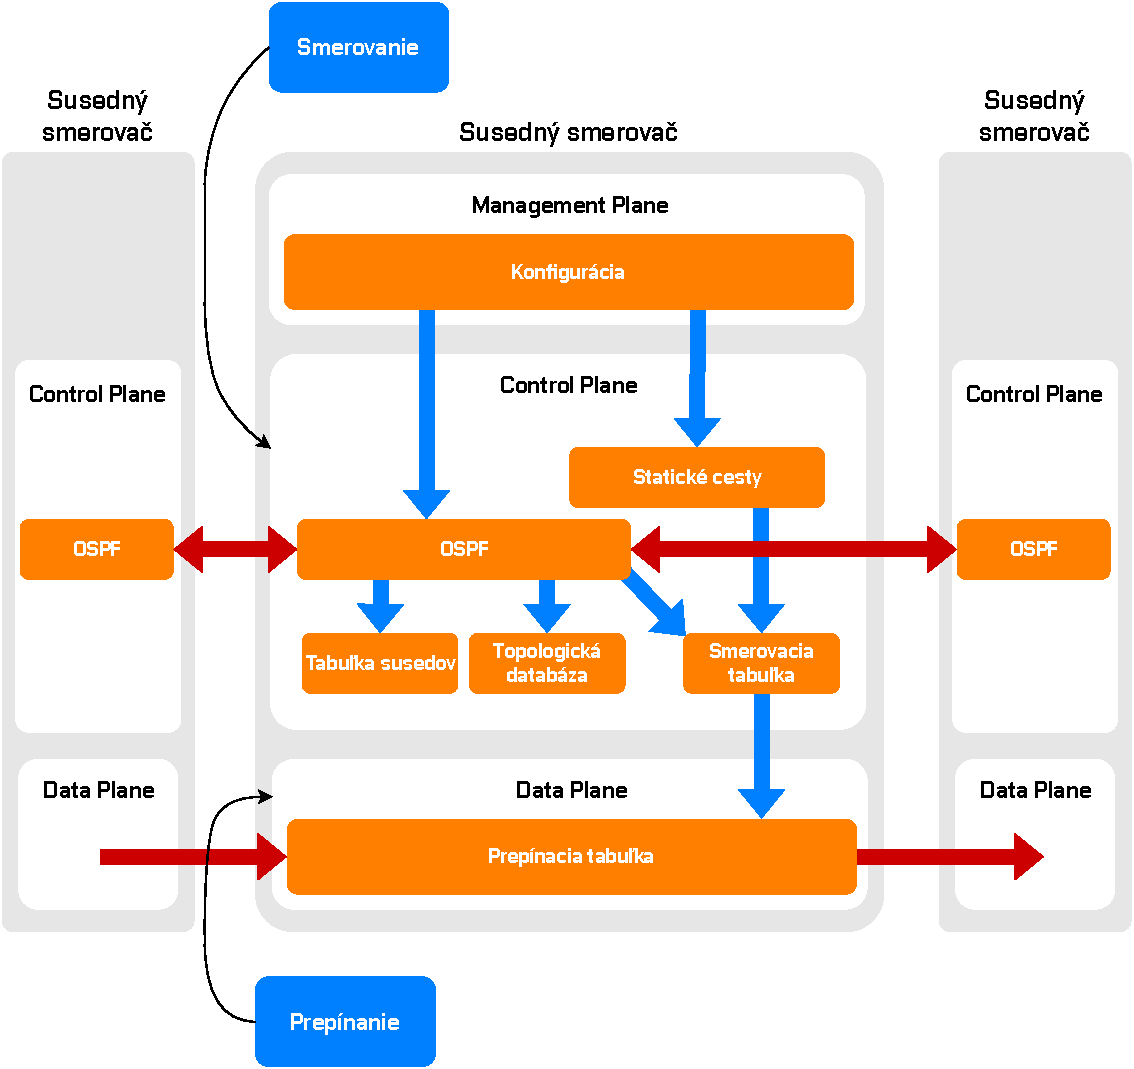
\includegraphics[scale=0.6]{obrazky/SDN_planes.pdf}
	\end{center}
	\caption[Rozdelenie rovín v smerovači, tok informácií v jeho vnútri a medzi susednými smerovačmi]{Rozdelenie rovín v smerovači, tok informácií v jeho vnútri a medzi susednými smerovačmi \cite{Pepelnjak2013}}
	\label{fig:sdn-planes}
\end{figure} 


\section{Prevázkové a bezpečnostné postupy}

\subsection*{Riadenie a zneužitie prístupu k manažmentu zariadenia}
Kritickým miestom často absentujúcim zabezpečenie je prístup ku konfigurácií zariadenia. Typickým príkladom je využitie protokolu \texttt{Telnet}, ktorý nešifruje spojenie a je teda ľahko odpočúvateľný. Preto sa odporúča využívať protokol \zk{zkSSH}, naviac je dobré využiť bezpečnú verziu 2 s rozumnou dĺžkou kľúča odpovedajúcou aktuálnym odporúčaniam. Jedným z opatrení na zabezpečenie SSH prístupu je zmena portu, na ktorom obvykle počúva z dôvodu, že útočník skúša periodicky útoky hrubou silou na \zkratka{zkTCP} port 22. Alternatívou na zabezpečenie SSH prístupu môže byť port knocking, ktorý na základe autorizácie dynamicky povolí záznam v ACL k portu, na ktorom počúva SSH.

Pri pokusoch o prihlásenie sa často využíva hádanie hesiel, preto je dobré určiť maximálny počet neúspešných pokusov a definovať čas po ktorý bude prihlásenie zablokované.

Riadenie prístupu k manažmentu zariadení by malo byť výhradne z obmedzeného rozsahu staníc administrátorov, na to poslúžia obmedzenia pomocou \zk{zkACL}, aby neprišlo k nechcenému prihláseniu alebo útoku \zk{zkDoS} z nechcených klientský staníc. Je tiež dobré zaznamenávať neúspešné ale aj úspešné prihlásenia do manažmentu zariadenia. 

V prípade konfigurácie viacerými administrátormi naraz môže vzniknúť konflikt, a preto je dobré zabezpečiť, aby v jednom okamihu mohol zmeny vykonávať iba jeden administrátor. Problémom môžu byť aj dlhé aktívne pripojenie k manažmentu zariadenia, ktoré môže byť zneužité pri odblokovanom počítači administrátora. 

Pri pokuse o prihlásenie alebo zmene nastavení je dobré informovať oznámením alebo správou potenciálneho útočníka s následkami, ktoré mu hrozia v prípade zneužitia zariadenia. 

\begin{figure}[H]
	\begin{center}
		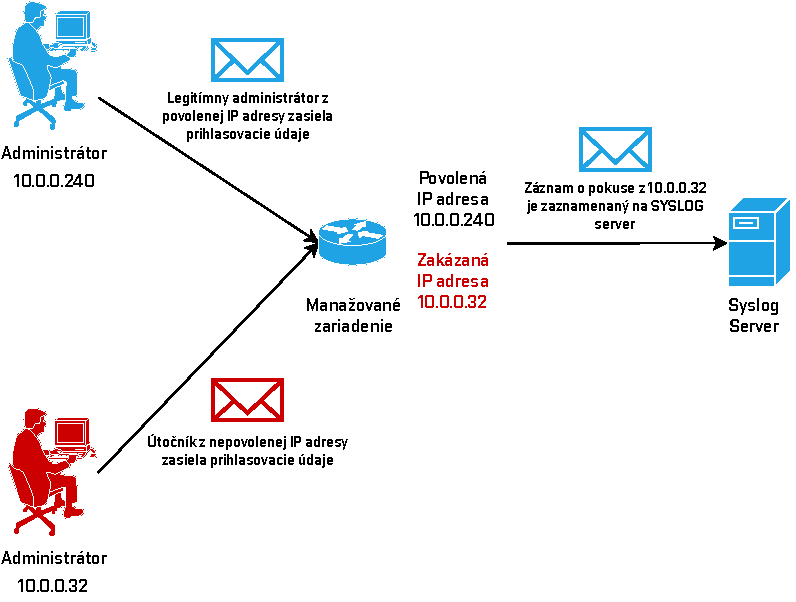
\includegraphics[scale=1]{obrazky/login-log.pdf}
	\end{center}
	\caption[Prihlasovanie k manažmentu zariadenia z povolených IP adries a logovanie pokusov z nepovolených IP adries]{Prihlasovanie k manažmentu zariadenia z povolených IP adries a logovanie pokusov z nepovolených IP adries}
	\label{fig:login-log-mngmt}
\end{figure} 

\newpage
Ďalšou obranou proti nechcenému prístupu na sieťové prvky je vytvorenie lokálnych účtov, ktoré budú použité na prihlasovanie a pri zmenách konfigurácie. Bez znalosti kombinácií mena a hesla by nemalo byť umožnené zmeniť nastavenia zariadenia.  

Najlepším riešením pre riadenie prístupu k manažmentu zariadenia a účtovaniu sú protokoly spadajúce do skupiny \zk{zkAAA}. Patria sem protokoly \texttt{Radius}, \texttt{TACACS+} alebo \texttt{Kerberos}. Tieto protokoly umožňujú okrem riadenia prihlásení administrátorov taktiež špecifikovať príkazy konfigurácie, ktoré budú jednotlivcom povolené a tiež zaznamenávať zmeny jednotlivých administrátorov v konfigurácií, ktoré učinili a taktiež kedy boli na zariadení prihlásení. Zároveň je treba určiť aj mechanizmus prihlásenia pri výpadku autentizačného serveru.

\begin{figure}[H]
	\begin{center}
		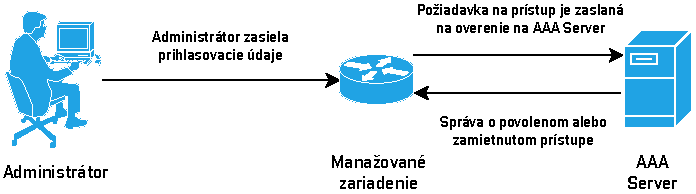
\includegraphics[scale=1.1]{obrazky/AAA.pdf}
	\end{center}
	\caption[Overenie prihlásenia k manažmentu zariadenia pomocou AAA serveru]{Overenie prihlásenia k manažmentu zariadenia pomocou AAA serveru}
	\label{fig:aaa-mngmt}
\end{figure} 



\subsection*{Filtrovanie prevádzky}
111,112
\section*{Smerovacie protokoly}
%TODO virtual link, auto summary
Používaním dynamických smerovacích protokolov prichádza sieť o určitú časť bezpečnosti a to vysielaním informácií o pripojených a naučených sieťach a cestách, ktoré môže útočník odchytávať. K tomu sa ešte môže pridať vloženie falošnej informácie a teda zaistenie smerovania cez útočníka. Našťastie obrana proti týmto útokom existuje, aj keď nie je vždy ideálna. V prípade vloženia informácie alebo cesty do správ, ktoré si vymieňajú dynamické smerovacie protokoly je možnou obranou autentizácia správ poslaných medzi smerovačmi. Pri zasielaní sa používa hash hesla a to sa pri prijatí druhým smerovačom porovná s vopred definovaným. Na obrázku \ref{fig:passive-int} je vidno, že informácie dynamického smerovacieho protokolu sú zastavené na pasívnom rozhraní, a teda užívatelia alebo útočník nemá možnosť sa tieto údaje dozvedieť.

\begin{figure}[H]
	\begin{center}
		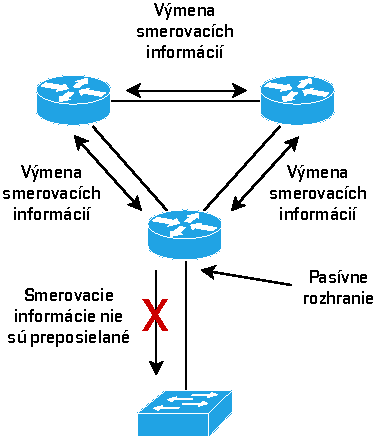
\includegraphics[scale=1]{obrazky/passive-interface.pdf}
	\end{center}
	\caption[Blokovanie správ dynamického smerovacieho protokolu na pasívne rozhranie]{Blokovanie správ dynamického smerovacieho protokolu na pasívne rozhranie}
	\label{fig:passive-int}
\end{figure} 

Bezpečnostnou hrozbou môže byť aj smerovanie na základe zdrojove adresy, pri ktorej si zdroj určí cestu, ktorou bude paket prechádzať namiesto aby túto skutočnosť prenechal na rozhodnutí smerovačov po ceste k cieľu. Táto funkcia využíva pole \texttt{IP Options}, ktoré býva však často ignorované prípadne pakety s týmto polom zahadzované z bezpečnostných dôvodov. Existujú dva módy, a to Strict a Loose, v prvom prípade musí paket prejsť všetkými definovanými bodmi a žiadnym iným. Naopak mód Loose definuje uzly ,ktoré je potreba navštíviť, no zároveň môžu byť navštívené aj iné uzly po ceste.  

Podvrhnutie IP adresy, tzv. IP spoofing je jedným z útokov, ktorým musia smerovače čeliť. Dá sa mu zbrániť pomocou \zkratka{zkURPF}, ktorý funguje buď v Strict alebo Loose móde a zisťuje prítomnosť zdrojovej zdrojovej IP adresy. Ako už názov napovedá, tak mód Strict je prísnejší, pretože zahadzuje pakety, ktorej zdrojová adresa sa nenachádza v smerovacej tabuľke a zároveň testuje či zdrojová adresa je dosiahnuteľná cez rozhranie, na ktorom bol paket prijatý. Tento mód je preto nevhodný pri asymetrickom smerovaní. Mód Loose testuje prítomnosť zdrojovej adresy iba v smerovacej tabuľke. 

Protokol \zkratka{zkBGP} okrem autentizácie obsahuje aj ďalšiu ochranu a to \zkratka{zkTTL} security \cite{AlHFaPbj6IbKzbuv}. Pri tomto prístupe sa porovnáva hodnota poľa TTL v pakete, ktorý dorazí do smerovača a známy počet skokov, ktorý sa nakonfiguruje medzi našim smerovačom a zdrojom. Mohlo by sa zdať, že priamo pripojené siete, teda susedné autonómne systémy týmto problémom netrpia, no pole TTL sa dá zmeniť tak, aby po príchode na smerovač obete malo toto pole hodnotu 1, čo je predvolené TTL, ktoré zasiela BGP, viď obrázok \ref{fig:ttl-sec}. Z tohto dôvodu sa používa obrátená forma kontroly, a to testovanie voči maximálnej hodnote TTL, čo je hodnota 255. To znamená, že všetky pakety od priamo pripojených BGP susedov budú mať po príchode na náš smerovač hodnotu TTL 255, tie ktoré to nebudú splňovať sú brané ako nelegitímne pakety, viď \ref{fig:ttl-sec}. Treba dodať, že v prípade že routery nie su priamo pripojené, tak je možné použiť aj definovanie vzdialenosti medzi smerovačmi, teda počet skokov, aby susedný smerovač dostal BGP správu. Bezpečnejšie je však použiť TTL security, tak že sa od čísla 255 odpočíta počet skokov medzi dvoma autonómnymi systémami a voči tejto hodnote sa bude robiť kontrola.

\begin{figure}[H]
	\begin{center}
		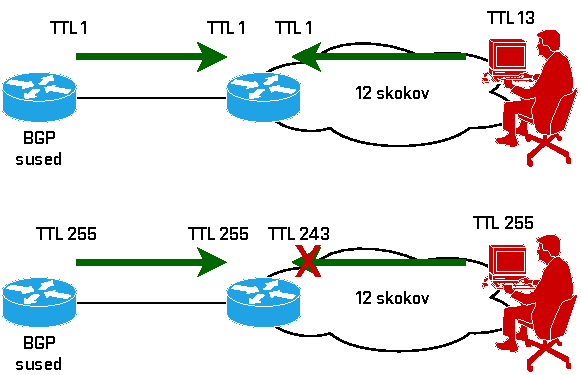
\includegraphics[scale=1]{obrazky/ttl-sec.pdf}
	\end{center}
	\caption[Porovnanie prístupov TTL security]{Porovnanie prístupov TTL security, kde sa v prvom prípade používa implicitná hodnota 1 na porovnanie TTL a v druhom prípade maximálna hodnota TTL \cite{AlHFaPbj6IbKzbuv}}
	\label{fig:ttl-sec}
\end{figure} 


\subsection*{Identifikácia zariadení, pravidiel a nastavení}
K lepšej identifikácií je dobrým pravidlom každé sieťové zariadenie vhodne pomenovať kombináciou typu zariadenie, vrstvy hierarchického modelu, na ktorej operuje a prípadne umiestnenia v racku, napríklad \texttt{sw01-dist-rack1}. V súvislosti s týmto nastavením sa často nastavuje aj doména, v ktorej je zariadenie umiestnené. Tieto dve prerekvizity potom umožňujú aj vzdialenú správu zariadenia.

Dôležitým prvkom sú komentáre k pravidlám v \zk{zkACL}, ktoré by mali nielen identifikovať, čo presne dané pravidlo povoľuje a zakazuje, ale aj identifikovať požiadavom, na základe ktorého bolo pravidlo vytvorené. 

Komentáre s popisom je dobré pridávať aj na rozhrania sieťových zariadení, napríklad s popisom, k akému zariadeniu dané rozhranie vedie. Posledným, ale nemenej dôležitým je pomenovanie \zk{zkVLAN} pre ich ľahšiu identifikáciu.

\subsection*{Šifrovanie hesiel}
Pri úniku konfigurácií môže dôjsť k odhaleniu hesiel uložených v nich, preto by mali byť v konfiguračnom súbore všetky heslá zahašované pomocou čo najpokročilejších hašovacích funkcií, ktoré dané zariadenie podporuje.

\subsection*{Logovanie}
Záznam činnosti zariadenia patrí k základným prvkom monitorovania sieťovej infraštruktúry spolu s notifikovaním o vzniknutých incidentoch. Na tieto účely sa používa prevažne dva protokoly, a to \zkratka{zkSNMP} a Syslog. 

Protokol SNMP využíva databázu MIB buď štandardizovanú, alebo rozšírenú daným výrobcom zariadenia. Jednotlivé monitorované objekty sú v tejto databáze organizované v stromovej štruktúre. V súčasnosti sa využívajú prevažne SNMP verzie 2c a 3. Je vysoko odporúčané využívať verziu 3, ktorá zabezpečuje ako integritu, tak aj dôvernosť a autentizáciu. Protokol SNMP umožňuje pomocou jednotlivých objektov meniť nastavenia zariadení, túto funkciu je však dobré vypnúť a povoliť iba čítanie objektov z presne definovaných IP adries pomocou ACL a asynchrónne správy TRAP.   

Druhou možnosťou monitorovania a notifikovania o incidentoch je protokol Syslog. Typicky sa nastavuje Syslog server, ktorý zbiera správy z viacerých zariadení, ktoré môžu byť následne spracovávané špeciálnymi programami a vizualizované v dohľadových centrách. Protokol Syslog pozná 8 úrovní dôležitosti (severity), pričom čím nižšie číslo dôležitosti, tým ide o závažnejší problém. Pri výpadku Syslog serveru je nutné záznamy ponechať na zariadení a preto mať dostatočné množstvo pamäte. V niektorých prípadoch môžu zariadenia vygenerovať väčšie množstvo správ, ktoré majú rovnaký čas a z tohto dôvodu by mali mať jednotlivé správy s rovnakým časom vzniku jednoznačné sekvenčné číslo, aby bolo možné zistiť postupnosť, v akom vznikli incidenty, napríklad zmeny v susedstvách dynamických smerovacích protokoloch.

Veľa útokov mieri práve na protokol SNMP, a preto ho mnohí odporúčajú vypínať, na druhej strane protokol Syslog nezabezpečuje žiadnu časť z triády CIA.   


\subsection*{Synchronizácia času}
Správny a aktuálny čas je dôležitý hlavne pre správne fungovanie certifikátov a protokolu Syslog. V prípade protokolu Syslog zabezpečuje jednoznačnú identifikáciu incidentu v správnom čase a teda lepšiu dohľadatelnosť a určenie vzniku problému. Keďže tento protokol využíva \zkratka{zkUDP}, tak je náchylný na DDoS reflektívne amplifikačné útoky. Tento typ útoku využíva krátku správu zasielanú na NTP server s podvrhnutou zdrojovou IP adresou (IP Spoofing), na ktorú budú zasielané odpovede s oveľa väčšou veľkosťou ako boli pôvodné správy na NTP server. Bohužiaľ obrana proti tomuto typu útoku je veľmi ťažká, poskytovatelia pripojenia k internetu sa s týmto neduhom väčšinou dokážu popasovať \cite{gTkmbyKon9H6tuAm}, v lokálnych sieťach môže pomôcť IP Snooping. Podľa Network Time Foundation \cite{s0goWNnWp5OjqREE}, aktuálna verzia protokolu 4 nepodporuje šifrovanie správ, no poskytuje akú-takú bezpečnosť pre koncových NTP klientov pomocou MD5 a to autentizáciu NTP serveru a kontrolu integrity. Naviac protokol nepodporuje žiadnu distribúciu kľúčov. Protokol NTP verzie 4 podopruje aj asymetrickú kryptografiu pomocou Autokey, no podpora tohto riešenia je veľmi slabá \cite{s0goWNnWp5OjqREE}, jedným z dôvodov je aj náročnosť výpočtov. NTP podporuje sťahovanie správ aj od klientov, toto je výhodné pri prerušení linky ku NTP serveru a na krížovú kontrolu času. Dôležitým nastavením je aj správne časové pásmo, ktoré je dobré zjednotiť naprieč všetkými spravovanými zariadeniami. V prípade roztrúsenia zariadení cez viacero časových pásiem je dobré využívať univerzálny čas UTC. Okrem protokolu NTP existuje niekoľko ďalších protokolov na synchronizáciu času, no sú menej používané. Príkladom je \zkratka{zkPTP}, ktorý je vhodný do lokálnych sietí kvôli vysokej presnosti. 

\begin{figure}[H]
	\begin{center}
		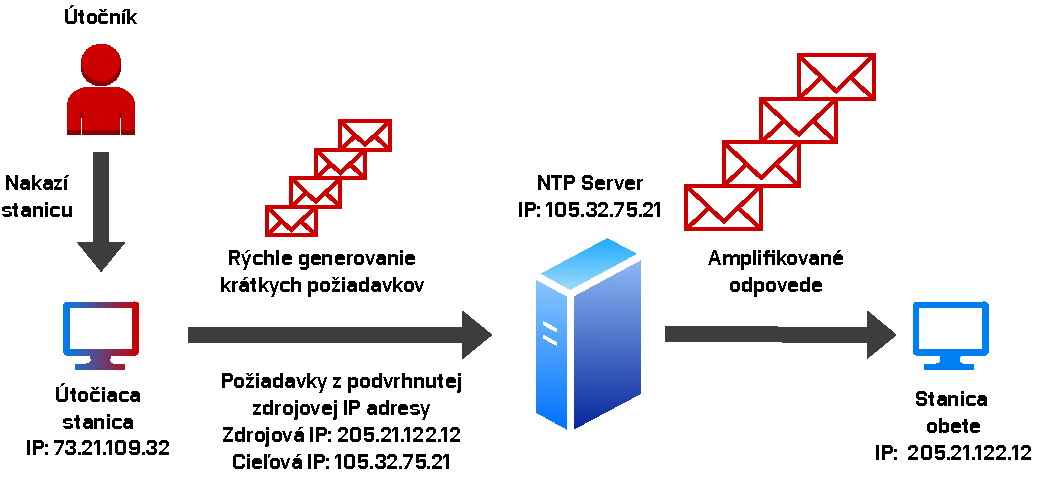
\includegraphics[scale=0.75]{obrazky/ntp_amplification.pdf}
	\end{center}
	\caption[Ilustrácia aplifikačného útoku cez nakazený počítač pomocou podvrhnutej IP adresy]{Ilustrácia aplifikačného útoku cez nakazený počítač pomocou podvrhnutej IP adresy \cite{gTkmbyKon9H6tuAm}}
	\label{fig:ntp-amp}
\end{figure} 

\subsection*{Záloha a zabezpečenie konfigurácií}
Konfigurácie zariadení a ich záloha sú veľmi dôležitým faktorom, ktorým sa treba zaoberať pri správe infraštruktúry. Pokiaľ sú prítomné aktuálne konfigurácie zariadení, tak pri výpadku hardware je možné ho vymeniť za nový a aplikovať fungujúcu konfiguráciu z poškodeného zariadenia zo zálohy. Zároveň by sa konfigurácia mala dostatočne zabezpečiť proti výmazu zo zariadenia a zálohovaného úložiska a dostatočne zabezpečiť. Zabezpečenie je dôležité, aby nedošlo k úniku konfigurácie útočníkom a nepovolaným osobám a následnému zneužitiu. Záloha konfigurácií by sa mala robiť cez zabezpečený kanál najlepšie pomocou protokolov podporujúcich šifrovanie, napríklad \zkratka{zkSCP} alebo \zkratka{zkSFTP} a nie pomocou \zkratka{zkTFTP}. Vhodná je aj prítomnosť záznamu zmien v konfigurácií v čase.

\subsection*{Správanie pri vysokom zaťažení}
V priebehu prevádzky sa môže vyskytnúť kratší alebo aj dlhý časový okamih, kedy je zariadenie vysoko zaťažené a nezvláda spracovávať požiadavky. Toto môže byť spôsobené útokom (D)DOS alebo nedostatočným dimenzovaním a zlou architektúrou siete. Aj napriek tomuto stavu by však malo byť zariadenie schopné odosielať chybové správy a notifikovať o problémoch. Zároveň by mali byť nastavené prahové hodnoty, ktoré budú indikovať stav, že môže dôjsť k nadmernému vyťaženiu procesoru, pamäti alebo linky či už pomocou Syslog správ alebo protokolu SNMP.

\subsection*{Monitorovanie výkonu siete}
Monitorovanie siete nie je len o chybových a operačných správach zariadení, ale aj o prevádzke, ktorá v sieti prebieha. Toto monitorovanie prevádzky musí byť vykonávané často z legislatívnych dôvodov a aplikuje sa u poskytovateľov pripojenia. Monitorovanie prevádzky sa však vykonáva aj v lokálnych sieťach, napríklad zrkadlením portov na analýzu útokov pre IDS alebo pre štatistické informácie a informácie o zaťažení pomocou protokolov sFlow a NetFlow.

\subsection*{Problémy vrstvy L2}
access, max, hopping, double tagging, blackhole, default access a trunk, dtp, spanning tree, dot1x, vtp
\subsection*{First Hop Security}
130 - 138 140 144-148 aj mac spoof a mac floof, teda spanning tree prikazy!!!
http://isp-servis.com/?p=191
\subsection*{First Hop Redundancy Protocols}
Protokoly na redundanciu brány štandardizovaný \zkratka{zkVRRP} a proprietárne \zkratka{zkHSRP} a \zkratka{zkGLBP} umožňujú využívať jednu virtuálnu adresu pre východziu bránu na koncových zariadeniach a tým sú pre toto koncové zariadenie transparentné. Naviac proprietárny protokol GLBP dokáže na ARP dotaz vracať ktorúkoľvek MAC adresu smerovača v skupine a tým rozkladať medzi ne záťaž. Všetky protokoly umožňujú autentizáciu správ zasielaných medzi sebou a tým istú úroveň bezpečnosti, aj keď nie úplne ideálnu.  

\subsection*{Tunely a VPN}
\zkratka{zkVPN} slúžia na vzdialené pripojenie zariadení, ktoré sú oddelené vonkajšou sieťou, internetom. Pre pripojenie vzdialených zariadení sa využívajú tunely. Spravidla sa VPN rozdeľujú na dva druhy, a to site-to-site, kde je pobačka k centrále pripojená cez hraničné prvky siete pomocou permanentne vytvoreného tunelu.  kde je vytvorené permanentné spojenie medzi hraničnými zariadeniami. Alebo druhou alternatívou je remote access VPN, kedy sa vytvára tunel na vyžiadanie a všetka sieťová prevádzka je môže byť smerovaná cez bod, ku ktorému sa stanica vzdialene pripája a zároveň je zariadeniu prístupná vnútorná sieť. Tieto tunely môžu byť šifrované, čo zabezpečuje dôvernosť a preto by mali byť preferovanou alternatívou. Dnes ešte stále používané protokoly \zkratka{zkPPTP}, \zkratka{zkL2TP} nie sú v dnešnej dobe považované za bezpečné. Preto sa dnes využívajú tunely pomocou protokolu \zkratka{zkIPSEC} prípadne pre remote access VPN je to protokol OpenVPN pracujúci na aplikačnej vrstve.

\begin{figure}[H]
	\begin{center}
		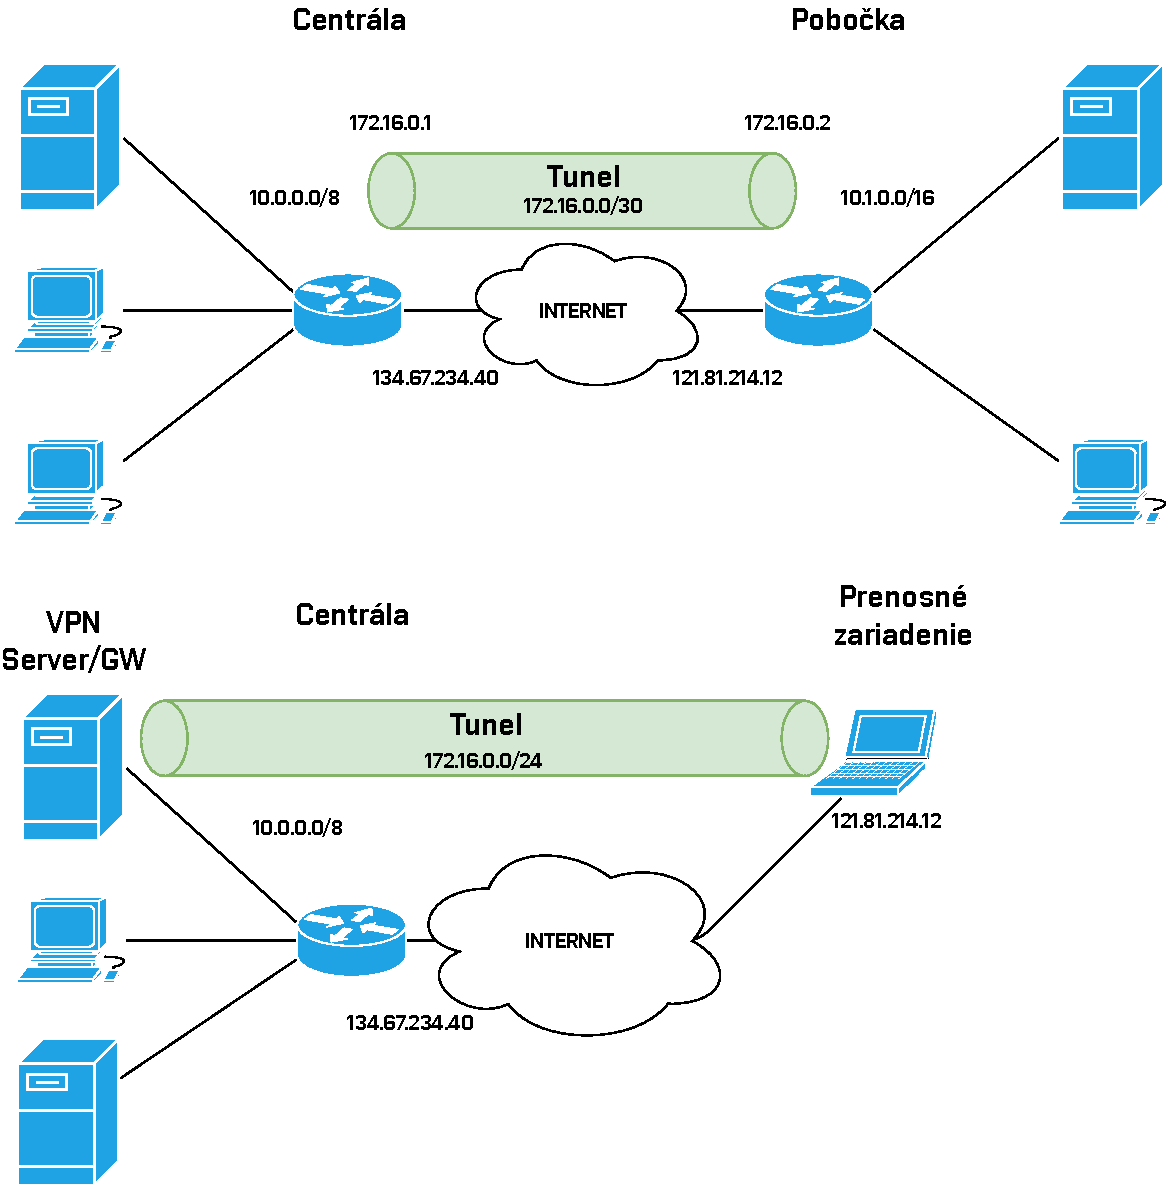
\includegraphics[scale=0.6]{obrazky/tunnels.pdf}
	\end{center}
	\caption[Porovnanie site-to-site a remote access VPN]{Porovnanie site-to-site a remote access VPN}
	\label{fig:tunnel}
\end{figure} 


\subsection*{Mapovanie siete a objavovanie zariadení}
Protokoly objavujúce zariadenia ako \zk{zkLLDP} a \zkratka{zkCDP} umožňujú získanie mnohých informácií o susedných pripojených zariadeniach, ako napríklad IP adresy, informácie o VLAN, operačnom systéme a mnohé ďalšie. Na tieto protokoly existuje veľké množstvo útokov s veľmi závažnými následkami. Častokrát sa tieto protokoly používajú pri IP telefónií a preto ich nie je možné plošne vypnúť, ideálne by sa mali zakázať aspoň na rozhraniach, kde nepotrebujú operovať. 

Získavanie smerovacích informácií a masku podsiete je možné aj pomocou správ \zkratka{zkICMP} typu redirects a mask reply. Problémom je aj directed broadcast, ktorý umožňuje získať ICMP odpoveď na správu ICMP Echo zaslanú na broadcast adresu smerovača. Zariadenia od spoločnosti Cisco majú túto funkciu už dlhšiu dobu z bezpečnostných dôvodov zakázanú. 

Mapovanie siete je možné aj pomocou \zkratka{zkMLD} a \zkratka{zkIGMP} Query správ, prípadne správami ICMP Echo na adresu ff02::1 a 224.0.0.1 \cite{Rey2016}\cite{Podermanski532015}. Na zabránenie tohto útoku je možné použiť pravidlá v ACL. 

Bezpečnostným problémom, ale aj systémom porušujúci fakt, že smerovač oddeľuje siete a broadcast doménu je proxy ARP. Tento systém umožňuje preposielanie ARP správ smerovačom do ďalších sietí. Využíva sa napríklad aj pri VPN, kedy chceme spojiť dve siete na vrstve sieťového rozhrania. 

\subsection*{Nepoužívané a nebezpečné služby}
Sieťové zariadenia sa často predávajú s rôznymi spustenými službami a tieto predvolené nastavenia, ktoré nie sú potrebné, môžu byť terčom útokov. Keďže administrátor tieto funkcie nepoužíva, tak im ani nevenuje pozornosť pri zabezpečovaní. Typickými príkladmi sú administrácia pomocou protokolu \zkratka{zkHTTP} prípadne spustený HTTP server a podobne. 

\subsection*{Ostatné}
Pre korektné fungovanie viacerých protokol je vhodné využívať ako zdroj Loopback rozhranie. Preto je dobrým zvykom definovať jedno Loopback rozhranie na zariadení, ktoré je dostupné hneď po štarte, nie ako fyzické rozhrania a môže byť užitočné ako identifikátor zariadenia pre viaceré protokoly. Toto rozhranie respektíve IP adresa sa používa ako zdrojová pri protokoloch \zkratka{zkNTP}, RADIUS, Tacacs+, \zk{zkSNMP}, Syslog, \zk{zkSSH} a tiež k identifikácií staníc dynamických smerovacích protokolov.

shutdown